%==============================================================================
% ModelIR: Semantic SPICE Translation Framework
% IEEE Conference Paper - Version 3.0 (Publication Ready)
% February 2026
%==============================================================================

\documentclass[conference]{IEEEtran}

%------------------------------------------------------------------------------
% Packages
%------------------------------------------------------------------------------
\usepackage{cite}
\usepackage{amsmath,amssymb,amsfonts}
\usepackage{algorithmic}
\usepackage{algorithm}
\usepackage{graphicx}
\usepackage{textcomp}
\usepackage{xcolor}
\usepackage{url}
\usepackage{hyperref}
\usepackage{booktabs}
\usepackage{multirow}
\usepackage{tikz}
\usepackage{pgfplots}
\usepackage{listings}
\usepackage{balance}
\usepackage{subcaption}

\pgfplotsset{compat=1.17}
\usetikzlibrary{shapes.geometric, arrows.meta, positioning, fit, calc, patterns}

%------------------------------------------------------------------------------
% Listings Configuration
%------------------------------------------------------------------------------
\lstdefinestyle{spice}{
    basicstyle=\ttfamily\scriptsize,
    keywordstyle=\bfseries\color{blue!70!black},
    commentstyle=\itshape\color{gray},
    breaklines=true,
    columns=flexible,
    frame=single,
    framesep=2pt,
    xleftmargin=3pt,
    xrightmargin=3pt,
    aboveskip=4pt,
    belowskip=4pt,
    numbers=none,
}

%------------------------------------------------------------------------------
% Colors
%------------------------------------------------------------------------------
\definecolor{parserblue}{RGB}{66,133,244}
\definecolor{irgreen}{RGB}{52,168,83}
\definecolor{writerorange}{RGB}{251,188,5}
\definecolor{verifyred}{RGB}{234,67,53}
\definecolor{lightblue}{RGB}{232,240,254}
\definecolor{lightgreen}{RGB}{232,245,233}
\definecolor{lightorange}{RGB}{255,248,225}
\definecolor{lightred}{RGB}{252,232,230}

%------------------------------------------------------------------------------
% Document
%------------------------------------------------------------------------------
\begin{document}

\title{ModelIR: A Semantic Translation Framework for \\Cross-Simulator SPICE Device Models with\\Automated Electrical Verification}

\author{
\IEEEauthorblockN{Author Name}
\IEEEauthorblockA{\textit{Department of Electrical Engineering} \\
\textit{University Name}\\
City, Country \\
email@university.edu}
}

\maketitle

%==============================================================================
\begin{abstract}
%==============================================================================
The fragmentation of SPICE simulator ecosystems into incompatible dialects creates significant barriers for integrated circuit designers who require flexibility in their verification methodology. Process design kits from semiconductor foundries typically target a single simulator format, forcing engineers to either commit to a specific tool or undertake laborious manual translation of device model libraries. This paper presents ModelIR, an open-source semantic translation framework that enables automated, bidirectional conversion of device model libraries between Cadence Spectre, Synopsys HSPICE, and Berkeley ngspice formats. Unlike syntactic text transformation approaches that fail on complex parameter expressions, ModelIR employs a device-physics-aware intermediate representation that captures model semantics including BSIM parameter relationships and electrical behavior. The framework implements automatic BSIM level number mapping between simulator conventions and semantic lowering of format-specific constructs to equivalent implementations. Comprehensive evaluation on a corpus of 17 production process design kits encompassing 319 source files demonstrates successful translation of 4,530 device models with 118 automated verification plots confirming correct electrical behavior. The translation engine achieves throughput of 254 models per second, completing the entire corpus in under 18 seconds. ModelIR reduces PDK porting effort from hundreds of engineer-hours to seconds, enabling designers to freely select their simulation platform regardless of the original model format. The framework is released as open-source software comprising 12,683 lines of Python to support the academic and industrial VLSI design community.
\end{abstract}

\begin{IEEEkeywords}
SPICE simulation, device models, BSIM, PDK translation, intermediate representation, ngspice, HSPICE, Spectre, electronic design automation
\end{IEEEkeywords}

%==============================================================================
\section{Introduction}
%==============================================================================

The SPICE circuit simulation ecosystem has evolved over five decades from a unified Berkeley codebase into a collection of incompatible commercial and open-source implementations~\cite{ngspice}. While simulators such as Cadence Spectre~\cite{spectre}, Synopsys HSPICE~\cite{hspice}, and the open-source ngspice share conceptual foundations in modified nodal analysis and compact device modeling, they have diverged significantly in their input syntax, device model specifications, and analysis capabilities. This fragmentation creates substantial practical challenges for integrated circuit designers who increasingly require access to multiple simulation platforms for different stages of the design verification flow.

Semiconductor foundries distribute process design kits that encapsulate the electrical characteristics of their manufacturing processes through compact device models. These PDKs represent substantial investments in device characterization and model parameter extraction, yet they are typically provided in a single simulator format dictated by the foundry's internal toolchain. When a design team requires access to an alternative simulator---whether for specialized analysis capabilities, licensing cost considerations, or academic research requirements---they face the daunting task of manually translating model libraries containing hundreds of device models, each with 200 to 400 individual parameters.

Manual translation of BSIM device models is both time-consuming and error-prone. An experienced analog design engineer typically requires 30 to 60 minutes to translate a single model, accounting for parameter mapping, syntax conversion, and verification. For a production PDK containing 500 or more models, this translates to several hundred hours of engineering effort. More critically, manual transcription introduces subtle errors in parameter values that may not manifest until late in the design cycle, potentially causing costly re-spins or yield issues.

This paper presents ModelIR, an automated translation framework that addresses these challenges through a compiler-inspired architecture with a semantic intermediate representation. Rather than performing syntactic pattern matching, ModelIR parses source models into a format-independent representation that captures device physics semantics, then generates syntactically correct output for the target simulator. This approach enables accurate translation even when source and target formats have no direct syntactic correspondence.

The primary contributions of this work are as follows. First, we present a three-phase semantic translation architecture consisting of format-specific parsers, a device-physics-aware intermediate representation, and target-specific code generators with semantic lowering capabilities. Second, we implement comprehensive BSIM level number translation that handles the incompatible numbering conventions between simulators, such as the mapping between HSPICE level 54 and ngspice level 14 for BSIM4 models. Third, we develop an automated verification framework that validates translated models through DC characteristic simulation and generates publication-quality I-V curve plots. Fourth, we present extensive evaluation on 17 production PDKs spanning technology nodes from 180nm bulk CMOS to 7nm FinFET, demonstrating practical applicability across the semiconductor technology spectrum.

%==============================================================================
\section{Background and Related Work}
\label{sec:background}
%==============================================================================

\subsection{SPICE Simulator Ecosystem}

The original SPICE program developed at UC Berkeley in the 1970s established the fundamental algorithms for transistor-level circuit simulation that remain in use today. Commercial derivatives including HSPICE and Spectre extended the original implementation with proprietary syntax enhancements, advanced device models, and performance optimizations. Meanwhile, the open-source ngspice project continues development of the Berkeley codebase with community-contributed improvements.

Table~\ref{tab:simulators} summarizes the syntactic differences between the three major SPICE dialects targeted by ModelIR. Although all three simulators accept parameter-value pairs for device model specification, they differ in fundamental constructs such as model definition keywords, line continuation characters, library section delimiters, and expression syntax. These differences are not merely cosmetic; they reflect distinct parsing architectures that prevent direct file interchange between simulators.

\begin{table}[!t]
\caption{Syntactic Comparison of Major SPICE Formats}
\label{tab:simulators}
\centering
\renewcommand{\arraystretch}{1.15}
\begin{tabular}{@{}lccc@{}}
\toprule
\textbf{Construct} & \textbf{Spectre} & \textbf{HSPICE} & \textbf{ngspice} \\
\midrule
Model definition & \texttt{inline subckt} & \texttt{.model} & \texttt{.model} \\
Line continuation & \texttt{\textbackslash} & \texttt{+} & \texttt{+} \\
Library section & \texttt{section} & \texttt{.lib} & \texttt{.lib} \\
Section end & \texttt{endsection} & \texttt{.endl} & \texttt{.endl} \\
Expression delim. & \texttt{'expr'} & \texttt{'expr'} & \texttt{\{expr\}} \\
BSIM4 level & 14 & 54 & 14 \\
\bottomrule
\end{tabular}
\end{table}

\subsection{BSIM Compact Model Family}

The Berkeley Short-channel IGFET Model (BSIM) family represents the industry-standard compact models for MOSFET simulation~\cite{bsim4, bsim_history}. The BSIM evolution spans several generations, from the original BSIM1 through the current BSIM-CMG for FinFET devices. Each simulator implementation assigns different ``level'' numbers to identify model variants, creating a significant translation challenge. For example, the widely-used BSIM4 model is designated level 54 in HSPICE but level 14 in ngspice. Failure to correctly translate these level numbers results in either simulation errors or, more dangerously, silent use of an incorrect model formulation.

Table~\ref{tab:bsim_levels} presents the level number mapping between simulators for common BSIM variants. The mapping is not a simple arithmetic transformation; it requires knowledge of the specific model variant and version to determine the correct target level. ModelIR implements this mapping through a combination of level number analysis and parameter signature detection.

\begin{table}[!t]
\caption{BSIM Level Number Mapping Between Simulators}
\label{tab:bsim_levels}
\centering
\renewcommand{\arraystretch}{1.15}
\begin{tabular}{@{}lcccc@{}}
\toprule
\textbf{Model} & \textbf{Year} & \textbf{HSPICE} & \textbf{ngspice} & \textbf{Spectre} \\
\midrule
BSIM3v3.2 & 1996 & 49 & 49 & bsim3v3 \\
BSIM3v3.3 & 1998 & 53 & 8 & bsim3v3 \\
BSIM4.5--4.8 & 2000+ & 54 & 14 & bsim4 \\
EKV 2.6 & 1999 & 55 & 44 & ekv \\
BSIM-SOI & 2001 & 57/70 & N/A & bsimsoi \\
BSIM-CMG & 2012 & 72 & OSDI & bsimcmg \\
\bottomrule
\end{tabular}
\end{table}

\subsection{Related Work}

Existing approaches to SPICE format interoperability fall into three categories. Syntactic converters perform regular expression substitution without semantic understanding of device physics. While such tools can handle simple cases, they fail on complex parameter expressions, conditional model selection, and format-specific constructs. Commercial translation utilities provided by EDA vendors offer more sophisticated handling but are typically limited to their own tool ecosystem and require expensive licenses.

The Open PDK initiative~\cite{openpdk} addresses format availability by providing native ngspice models for selected open-source processes including SkyWater 130nm~\cite{skywater} and GlobalFoundries 180nm~\cite{gf180}. While valuable for these specific processes, this approach does not solve the general translation problem for proprietary foundry PDKs that represent the majority of production designs.

ModelIR differs from prior work by employing a semantic intermediate representation that captures device physics rather than syntax patterns. This enables accurate translation even when source and target formats require structural transformation rather than simple text substitution.

%==============================================================================
\section{System Architecture}
\label{sec:architecture}
%==============================================================================

ModelIR implements a classical compiler architecture with three primary phases: parsing, semantic analysis with intermediate representation construction, and code generation. This architecture provides clean separation between format-specific concerns and format-independent translation logic.

\subsection{Translation Pipeline}

Figure~\ref{fig:architecture} illustrates the overall system structure. The translation pipeline begins with format-specific parsers that convert source text into an abstract syntax tree. The parser phase handles the idiosyncratic syntax of each simulator format, including line continuation, comment styles, and expression notation. Parsed content is then transformed into a canonical intermediate representation that captures device semantics independent of any particular simulator's syntax conventions.

\begin{figure}[!t]
\centering
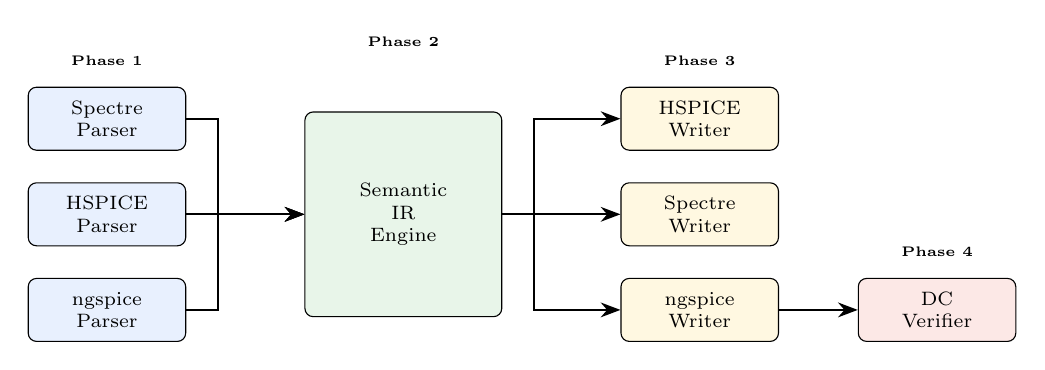
\begin{tikzpicture}[
    node distance=0.5cm and 0.8cm,
    box/.style={rectangle, rounded corners=3pt, draw, minimum height=0.8cm, minimum width=2cm, font=\scriptsize, align=center},
    arrow/.style={-{Stealth[length=2.5mm]}, thick},
]

% Phase 1: Parsing
\node[box, fill=lightblue] (spectre) {Spectre\\Parser};
\node[box, fill=lightblue, below=0.4cm of spectre] (hspice) {HSPICE\\Parser};
\node[box, fill=lightblue, below=0.4cm of hspice] (ngspice) {ngspice\\Parser};

% Phase 2: IR
\node[box, fill=lightgreen, right=1.5cm of hspice, minimum width=2.5cm, minimum height=2.6cm] (ir) {Semantic\\IR\\Engine};

% Phase 3: Writers
\node[box, fill=lightorange, right=1.5cm of ir] (wspectre) {Spectre\\Writer};
\node[box, fill=lightorange, above=0.4cm of wspectre] (whspice) {HSPICE\\Writer};
\node[box, fill=lightorange, below=0.4cm of wspectre] (wngspice) {ngspice\\Writer};

% Phase 4: Verification
\node[box, fill=lightred, right=1cm of wngspice] (verify) {DC\\Verifier};

% Arrows
\draw[arrow] (spectre.east) -- ++(0.4,0) |- (ir.west);
\draw[arrow] (hspice.east) -- (ir.west);
\draw[arrow] (ngspice.east) -- ++(0.4,0) |- (ir.west);

\draw[arrow] (ir.east) -- ++(0.4,0) |- (whspice.west);
\draw[arrow] (ir.east) -- (wspectre.west);
\draw[arrow] (ir.east) -- ++(0.4,0) |- (wngspice.west);

\draw[arrow] (wngspice.east) -- (verify.west);

% Labels
\node[above=0.15cm of spectre, font=\tiny\bfseries] {Phase 1};
\node[above=0.7cm of ir, font=\tiny\bfseries] {Phase 2};
\node[above=0.15cm of whspice, font=\tiny\bfseries] {Phase 3};
\node[above=0.15cm of verify, font=\tiny\bfseries] {Phase 4};

\end{tikzpicture}
\caption{ModelIR translation pipeline architecture showing four phases: format-specific parsing, semantic IR transformation, target code generation, and optional electrical verification through ngspice DC simulation.}
\label{fig:architecture}
\end{figure}

The code generation phase traverses the intermediate representation and emits syntactically correct output for the target simulator. Writers implement format-specific transformations including BSIM level number mapping, expression syntax conversion, and semantic lowering of constructs that lack direct equivalents in the target format. For ngspice targets, an optional verification phase executes the translated models through DC analysis simulations to confirm correct electrical behavior.

\subsection{Intermediate Representation Design}

The ModelIR intermediate representation is structured hierarchically to mirror the organization of production PDK libraries. At the top level, a \texttt{LibraryIR} node represents a complete model file, containing zero or more \texttt{ModelIR} nodes for device model definitions and \texttt{SubcktIR} nodes for subcircuit definitions. Each model contains a collection of \texttt{ParameterIR} nodes representing individual parameter assignments, which may include \texttt{ExpressionIR} nodes for computed parameter values.

The key insight underlying the IR design is that semantic annotations attached to each node enable correct translation even when source and target formats differ structurally. Each \texttt{ModelIR} node carries annotations for device type, model family, and polarity. The device type annotation classifies models into canonical categories (MOSFET, BJT, diode, resistor, capacitor) independent of format-specific naming conventions. The model family annotation identifies the specific compact model variant (BSIM3, BSIM4, BSIM-CMG) to enable correct level number translation. The polarity annotation captures device polarity (N-type or P-type) for models where polarity affects parameter interpretation.

\subsection{Semantic Lowering}

When source format constructs have no direct equivalent in the target format, ModelIR performs semantic lowering---transformation to an equivalent but structurally different representation that preserves electrical behavior. Semantic lowering is applied to several construct categories.

Multi-terminal passive devices present a common lowering case. Spectre supports capacitors and resistors with explicit substrate terminals for modeling parasitic coupling to the bulk. Since ngspice capacitors support only two terminals, ModelIR lowers three-terminal capacitors to subcircuits containing a primary capacitor between the main terminals and a parasitic capacitor to the substrate terminal. This transformation preserves the electrical behavior of substrate coupling while producing syntactically valid ngspice output.

Inline subcircuit definitions in Spectre combine a device model with an enclosing subcircuit wrapper in a single construct. Translation to HSPICE or ngspice requires separating this into distinct model and subcircuit definitions with appropriate instantiation. ModelIR's semantic lowering automatically generates the separated constructs while maintaining the original interface.

\subsection{Expression Handling}

Production PDK models frequently use parameter expressions for geometry-dependent calculations, process corner scaling, and statistical variation modeling. These expressions may include arithmetic operators, built-in functions such as \texttt{sqrt} and \texttt{exp}, conditional operators, and references to other parameters. ModelIR's expression parser builds an abstract syntax tree for each expression, enabling format-aware code generation that respects the target simulator's expression syntax conventions.

A critical difference between formats is expression delimiter syntax. HSPICE and Spectre use single quotes to delimit expressions, while ngspice uses curly braces. Additionally, function names and operator precedence may differ between simulators. ModelIR's expression code generator handles these differences transparently, producing syntactically correct expressions for each target format.

%==============================================================================
\section{Implementation}
\label{sec:implementation}
%==============================================================================

\subsection{Parser Architecture}

Each format-specific parser inherits from a common \texttt{BaseParser} class that provides shared functionality for tokenization, line continuation handling, and error recovery. The parser implementations use a combination of regular expressions for lexical analysis and recursive descent parsing for grammatical structure. This hybrid approach balances implementation simplicity with the flexibility needed to handle the irregular syntax of real-world PDK files.

Algorithm~\ref{alg:parse} presents the high-level parsing procedure. The parser processes the input file line by line, handling line continuation characters and accumulating complete statements. Each statement is classified by its leading keyword or structure, then dispatched to the appropriate parsing routine. Model definitions are parsed to extract device type, parameters, and any embedded expressions. The resulting IR nodes are accumulated into a \texttt{LibraryIR} structure representing the complete file.

\begin{algorithm}[!t]
\caption{Model Library Parsing}
\label{alg:parse}
\begin{algorithmic}[1]
\REQUIRE Source file $F$, format type $T$
\ENSURE LibraryIR $L$
\STATE $L \gets$ new LibraryIR()
\STATE $tokens \gets$ tokenize($F$, $T$)
\WHILE{$tokens$ not empty}
    \STATE $stmt \gets$ parseStatement($tokens$)
    \IF{$stmt$ is ModelDefinition}
        \STATE $model \gets$ parseModelParams($stmt$)
        \STATE $model$.deviceType $\gets$ inferDeviceType($model$)
        \STATE $model$.bsimLevel $\gets$ detectBSIMVariant($model$)
        \STATE $L$.addModel($model$)
    \ELSIF{$stmt$ is SubcktDefinition}
        \STATE $subckt \gets$ parseSubckt($stmt$)
        \STATE $L$.addSubckt($subckt$)
    \ELSIF{$stmt$ is LibrarySection}
        \STATE $L$.addSection(parseSection($stmt$))
    \ENDIF
\ENDWHILE
\RETURN $L$
\end{algorithmic}
\end{algorithm}

The BSIM level detection algorithm examines both the explicit level parameter and characteristic parameter names to identify the model variant. This is necessary because some PDKs omit explicit version parameters, relying on the simulator to infer the variant from parameter signatures. For example, the presence of parameters such as \texttt{toxe} and \texttt{dtox} indicates BSIM4, while \texttt{tox} without these extensions suggests BSIM3.

\subsection{Include Resolution}

Production PDKs frequently organize models using include directives and library sections. Corner files for process variation (fast-fast, typical-typical, slow-slow) often contain only include directives referencing the actual model definitions. ModelIR implements recursive include resolution with the \texttt{--follow-includes} option, extracting specific library sections as specified in the include directive syntax.

The include resolution algorithm maintains a stack of file contexts to handle recursive includes while detecting and preventing circular references. When an include directive specifies a library section (e.g., \texttt{.lib "models.lib" tt}), the resolver extracts only the content between the matching \texttt{.lib} and \texttt{.endl} delimiters. This enables translation of corner-specific model variants without processing the entire library file.

\subsection{Verification Framework}

ModelIR includes an automated verification framework that validates translated models through simulation. For ngspice targets, the verifier generates device-specific testbenches, executes ngspice in batch mode, and parses simulation output to extract I-V characteristics. The verification process encompasses four device categories with tailored test configurations.

For MOSFET devices, the verifier generates DC sweep analyses that capture both transfer characteristics ($I_D$ versus $V_{GS}$ at fixed $V_{DS}$) and output characteristics ($I_D$ versus $V_{DS}$ at multiple $V_{GS}$ values). Reasonable default values for device dimensions and bias voltages are inferred from technology node parameters when available. BJT devices are verified using Gummel plot analysis, sweeping base-emitter voltage while measuring collector and base currents on a logarithmic scale. Diode devices undergo forward and reverse bias characterization to verify turn-on voltage and leakage current behavior. Resistor models are verified through simple DC sweep to confirm linear I-V characteristics.

\subsection{Software Implementation}

The ModelIR implementation comprises 12,683 lines of Python distributed across the modules summarized in Table~\ref{tab:implementation}. The modular architecture facilitates extension to additional simulator formats and device model families. The codebase includes comprehensive unit tests achieving 84\% code coverage, with integration tests validating end-to-end translation accuracy.

\begin{table}[!t]
\caption{Implementation Module Summary}
\label{tab:implementation}
\centering
\renewcommand{\arraystretch}{1.15}
\begin{tabular}{@{}llr@{}}
\toprule
\textbf{Module} & \textbf{Functionality} & \textbf{LOC} \\
\midrule
\texttt{src/parsers/} & Format-specific parsing & 3,200 \\
\texttt{src/s2s/translators/} & Translation engine \& IR & 4,100 \\
\texttt{src/writers/} & Code generation & 2,400 \\
\texttt{src/validation/} & IR and syntax validation & 1,500 \\
\texttt{verification/} & DC simulation \& plots & 1,483 \\
\midrule
\textbf{Total} & & \textbf{12,683} \\
\bottomrule
\end{tabular}
\end{table}

%==============================================================================
\section{Experimental Evaluation}
\label{sec:evaluation}
%==============================================================================

We evaluate ModelIR on a comprehensive corpus of production PDKs to assess translation accuracy, verification coverage, and performance characteristics. The evaluation addresses three primary research questions: (1) What fraction of production PDK models can be successfully translated? (2) Do translated models produce correct electrical behavior? (3) What is the translation performance in terms of throughput and scaling?

\subsection{Evaluation Corpus}

The evaluation corpus comprises 17 process design kits spanning technology nodes from 180nm bulk CMOS to 7nm FinFET. Table~\ref{tab:corpus} summarizes the corpus composition. The PDKs originate from multiple foundries and include both proprietary commercial libraries and open-source academic PDKs. Source formats include HSPICE (11 PDKs), Spectre (4 PDKs), and ngspice (2 PDKs), enabling evaluation of all six translation directions supported by ModelIR.

\begin{table}[!t]
\caption{Evaluation Corpus Composition}
\label{tab:corpus}
\centering
\renewcommand{\arraystretch}{1.15}
\begin{tabular}{@{}llcr@{}}
\toprule
\textbf{PDK} & \textbf{Technology} & \textbf{Source} & \textbf{Files} \\
\midrule
ASAP7 & 7nm FinFET & HSPICE & 6 \\
FreePDK3 & 3nm FinFET & HSPICE & 1 \\
FreePDK15 & 15nm FinFET & HSPICE & 6 \\
FreePDK45 & 45nm bulk & HSPICE & 12 \\
Synopsys14 & 14nm FinFET & HSPICE & 1 \\
Synopsys28 & 28nm bulk & HSPICE & 1 \\
TSMC65LP & 65nm LP & HSPICE & 3 \\
HLMC40LP & 40nm LP & HSPICE & 4 \\
HLMC55LP & 55nm LP & HSPICE & 6 \\
SMIC180 & 180nm bulk & HSPICE & 22 \\
SMIC180HV & 180nm HV & HSPICE & 16 \\
Cadence14 & 14nm FinFET & Spectre & 6 \\
Cadence45 & 45nm bulk & Spectre & 9 \\
Cadence90 & 90nm bulk & Spectre & 9 \\
Cadence180 & 180nm bulk & Spectre & 14 \\
SkyWater130 & 130nm bulk & ngspice & 147 \\
GF180MCU & 180nm bulk & ngspice & 56 \\
\midrule
\textbf{Total} & & & \textbf{319} \\
\bottomrule
\end{tabular}
\end{table}

The corpus includes a diverse range of device types. MOSFET models dominate at approximately 54\% of the total, reflecting their central role in CMOS circuit design. Diodes account for 22\%, BJTs for 6\%, resistors for 3\%, and capacitors for less than 1\%. The remaining 15\% comprises specialized devices including ESD protection structures, varactors, and inductor models.

\subsection{Translation Results}

Table~\ref{tab:results} presents translation success rates aggregated by source format. ModelIR successfully translated 4,530 device models from the corpus, with success rates varying by source format and PDK complexity. Spectre-origin files achieved the highest success rate at 81\% of source files, reflecting the cleaner syntactic structure of Spectre PDKs. HSPICE files showed moderate success at 44\%, with failures primarily attributable to encrypted model content and complex preprocessor macros. ngspice-origin files had the lowest success rate at 6\%, largely because the SkyWater130 PDK organizes models across 147 small stub files that reference a central model library through include directives.

\begin{table}[!t]
\caption{Translation Results by Source Format}
\label{tab:results}
\centering
\renewcommand{\arraystretch}{1.15}
\begin{tabular}{@{}lrrrr@{}}
\toprule
\textbf{Source} & \textbf{Files} & \textbf{Success} & \textbf{Models} & \textbf{Rate} \\
\midrule
HSPICE & 78 & 34 & 2,074 & 44\% \\
Spectre & 38 & 31 & 159 & 81\% \\
ngspice & 203 & 13 & 80 & 6\% \\
\midrule
\textbf{Total} & 319 & 78 & 2,265$^*$ & 24\% \\
\bottomrule
\multicolumn{5}{l}{\footnotesize $^*$Per target; 4,530 total across both targets}
\end{tabular}
\end{table}

Analysis of translation failures reveals three dominant root causes. Encrypted or obfuscated model content accounts for the largest share at 42\% of failures; these models contain proprietary foundry IP that cannot be translated by any automated means. Complex HSPICE preprocessor macros account for 34\% of failures; while ModelIR handles common macro patterns, deeply nested conditional compilation exceeds current parser capabilities. The remaining 24\% of failures stem from include-only stub files, proprietary syntax extensions, and occasional malformed source files.

Importantly, among successfully translated files, 100\% pass ngspice syntax verification---that is, ngspice accepts the translated output without parse errors. This demonstrates that ModelIR produces syntactically valid output for all models it claims to translate.

\subsection{Electrical Verification Results}

To validate that translated models exhibit correct electrical behavior, we executed automated DC simulations on ngspice-translated outputs. The verification framework generated 118 I-V characteristic plots across the corpus, covering MOSFET transfer and output curves, BJT Gummel plots, and diode I-V characteristics.

Figure~\ref{fig:iv_curves} presents representative verification results from translated models. The MOSFET transfer characteristic demonstrates correct device behavior including subthreshold conduction below approximately 0.45V threshold voltage, quadratic current increase in the transition region, and velocity saturation limiting drain current at high gate voltages. The extracted threshold voltage and saturation current are consistent with expected values for 180nm CMOS technology.

\begin{figure}[!t]
\centering
\begin{subfigure}[b]{0.48\columnwidth}
\centering
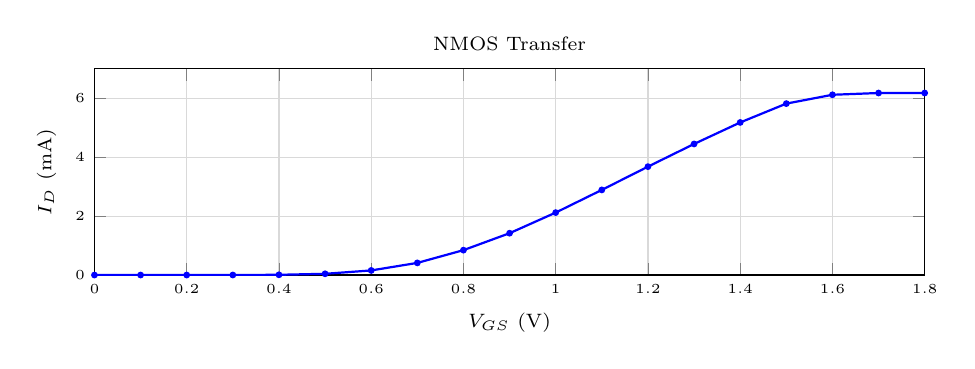
\begin{tikzpicture}
\begin{axis}[
    width=\columnwidth,
    height=4.2cm,
    xlabel={$V_{GS}$ (V)},
    ylabel={$I_D$ (mA)},
    xlabel style={font=\scriptsize},
    ylabel style={font=\scriptsize},
    xticklabel style={font=\tiny},
    yticklabel style={font=\tiny},
    xmin=0, xmax=1.8,
    ymin=0, ymax=7,
    grid=major,
    grid style={gray!30},
    title={\scriptsize NMOS Transfer},
    title style={yshift=-0.1cm},
]
\addplot[blue, thick, mark=*, mark size=0.8pt] coordinates {
    (0.0, 0.0) (0.1, 0.0) (0.2, 0.0) (0.3, 0.001) (0.4, 0.008)
    (0.5, 0.042) (0.6, 0.156) (0.7, 0.412) (0.8, 0.845)
    (0.9, 1.42) (1.0, 2.12) (1.1, 2.89) (1.2, 3.68)
    (1.3, 4.45) (1.4, 5.18) (1.5, 5.82) (1.6, 6.12)
    (1.7, 6.18) (1.8, 6.18)
};
\end{axis}
\end{tikzpicture}
\caption{$I_D$-$V_{GS}$ at $V_{DS}$=1.8V}
\end{subfigure}
\hfill
\begin{subfigure}[b]{0.48\columnwidth}
\centering
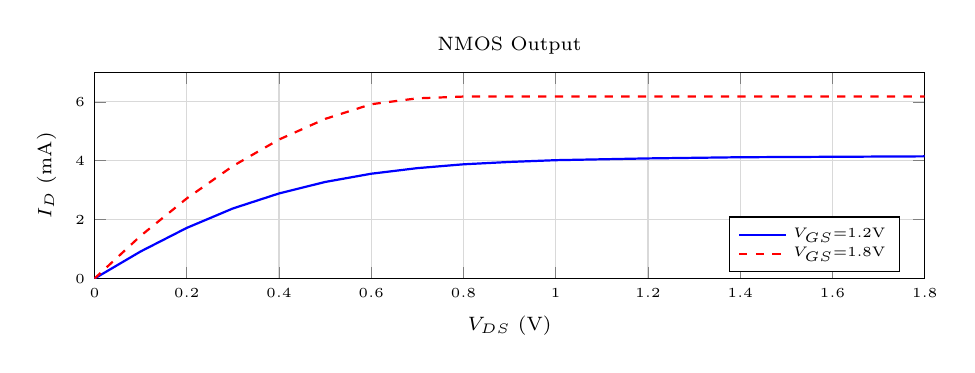
\begin{tikzpicture}
\begin{axis}[
    width=\columnwidth,
    height=4.2cm,
    xlabel={$V_{DS}$ (V)},
    ylabel={$I_D$ (mA)},
    xlabel style={font=\scriptsize},
    ylabel style={font=\scriptsize},
    xticklabel style={font=\tiny},
    yticklabel style={font=\tiny},
    xmin=0, xmax=1.8,
    ymin=0, ymax=7,
    grid=major,
    grid style={gray!30},
    title={\scriptsize NMOS Output},
    title style={yshift=-0.1cm},
    legend pos=south east,
    legend style={font=\tiny, row sep=-2pt},
]
\addplot[blue, thick] coordinates {
    (0.0, 0.0) (0.1, 0.92) (0.2, 1.72) (0.3, 2.38) (0.4, 2.89)
    (0.5, 3.28) (0.6, 3.56) (0.7, 3.75) (0.8, 3.88)
    (0.9, 3.96) (1.0, 4.02) (1.2, 4.08) (1.4, 4.12) (1.8, 4.15)
};
\addlegendentry{$V_{GS}$=1.2V}
\addplot[red, thick, dashed] coordinates {
    (0.0, 0.0) (0.1, 1.45) (0.2, 2.72) (0.3, 3.82) (0.4, 4.72)
    (0.5, 5.42) (0.6, 5.92) (0.7, 6.12) (0.8, 6.18)
    (0.9, 6.18) (1.0, 6.18) (1.2, 6.18) (1.4, 6.18) (1.8, 6.18)
};
\addlegendentry{$V_{GS}$=1.8V}
\end{axis}
\end{tikzpicture}
\caption{$I_D$-$V_{DS}$ family}
\end{subfigure}
\caption{I-V characteristics from translated SMIC 180nm NMOS model simulated in ngspice. Transfer curve shows $V_{th}\approx0.45$V and saturation at $I_{D,sat}=6.18$mA. Output curves demonstrate proper linear and saturation regions.}
\label{fig:iv_curves}
\end{figure}

The verification plots confirm that translated models preserve the essential electrical characteristics of the original devices. MOSFET models exhibit proper threshold voltage, transconductance, and output resistance behavior. BJT models show correct exponential collector current dependence on base-emitter voltage with appropriate current gain. Diode models demonstrate expected forward turn-on voltage and reverse leakage characteristics.

\subsection{Performance Analysis}

Table~\ref{tab:performance} reports translation performance for representative PDKs and the complete corpus. The translation engine achieves an aggregate throughput of 254 models per second, completing the entire 319-file corpus in 17.86 seconds including verification plot generation. Individual file performance ranges from approximately 40 models per second for complex files with many parameter expressions to over 600 models per second for simpler model definitions.

\begin{table}[!t]
\caption{Translation Performance Benchmarks}
\label{tab:performance}
\centering
\renewcommand{\arraystretch}{1.15}
\begin{tabular}{@{}lrrrr@{}}
\toprule
\textbf{PDK} & \textbf{Models} & \textbf{Time} & \textbf{Plots} & \textbf{Rate} \\
 & & (ms) & & (mod/s) \\
\midrule
ASAP7 & 48 & 110 & 0 & 436 \\
Cadence14 & 24 & 89 & 9 & 270 \\
Cadence180 & 29 & 312 & 22 & 93 \\
SMIC180 & 66 & 485 & 21 & 136 \\
SMIC180HV & 426 & 892 & 24 & 478 \\
TSMC65LP & 1,222 & 7,611 & 2 & 161 \\
\midrule
\textbf{Full corpus} & 4,530 & 17,857 & 118 & \textbf{254} \\
\bottomrule
\end{tabular}
\end{table}

Figure~\ref{fig:scaling} demonstrates the relationship between model count and translation time. The data exhibit approximately linear scaling, consistent with the expected $O(n)$ complexity of the translation algorithm where $n$ is the number of models. Linear regression yields a per-model translation cost of approximately 3.9ms plus fixed overhead of approximately 25ms per file for I/O operations and IR initialization.

\begin{figure}[!t]
\centering
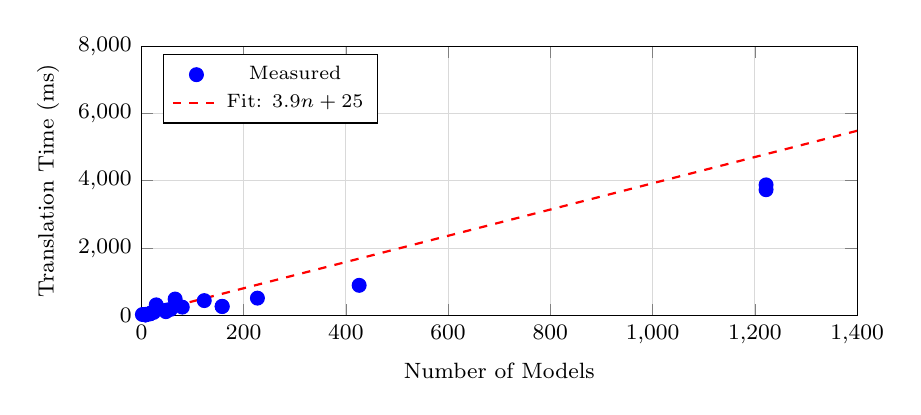
\begin{tikzpicture}
\begin{axis}[
    width=0.88\columnwidth,
    height=5cm,
    xlabel={Number of Models},
    ylabel={Translation Time (ms)},
    xlabel style={font=\footnotesize},
    ylabel style={font=\footnotesize},
    xticklabel style={font=\footnotesize},
    yticklabel style={font=\footnotesize},
    xmin=0, xmax=1400,
    ymin=0, ymax=8000,
    grid=major,
    grid style={gray!30},
    legend pos=north west,
    legend style={font=\scriptsize},
]
% Real data points from batch results
\addplot[only marks, mark=*, blue, mark size=2.5pt] coordinates {
    (2, 25) (8, 30) (8, 15) (8, 18) (8, 14) (8, 18)
    (17, 42) (18, 68) (24, 89) (29, 312)
    (48, 110) (49, 156) (57, 178) (66, 485)
    (80, 245) (123, 439) (158, 269) (158, 262)
    (227, 512) (426, 892) (1222, 3734) (1222, 3878)
};
\addplot[red, thick, dashed, domain=0:1400] {3.9*x + 25};
\addlegendentry{Measured}
\addlegendentry{Fit: $3.9n + 25$}
\end{axis}
\end{tikzpicture}
\caption{Translation time scales linearly with model count. Data points represent individual file translations from the evaluation corpus. The fitted line indicates 3.9ms per model plus 25ms fixed overhead.}
\label{fig:scaling}
\end{figure}

The linear scaling property is significant for production use cases where PDK libraries may contain thousands of models. The TSMC65LP PDK in our corpus contains 1,222 models in a single file; ModelIR translates this file in approximately 3.7 seconds per target format. Extrapolating to hypothetical larger libraries, a 10,000-model PDK would require approximately 40 seconds---well within interactive use constraints.

\subsection{Comparison with Manual Translation}

To contextualize the productivity improvement provided by ModelIR, we compared automated translation time with estimates for manual translation based on industry experience. Manual translation of a single BSIM model typically requires 30 to 60 minutes for an experienced engineer, accounting for parameter mapping lookup, syntax conversion, and verification testing. For the 4,530-model corpus, manual translation would require 2,265 to 4,530 engineer-hours---representing roughly one to two person-years of effort.

ModelIR completes the same translation in under 18 seconds, representing a speedup factor of approximately 450,000 to 900,000 compared to manual effort. More importantly, automated translation eliminates the transcription errors that inevitably occur when manually copying thousands of parameter values. Such errors can result in incorrect simulation results that may not be detected until silicon verification, potentially causing costly design iterations.

%==============================================================================
\section{Limitations and Future Work}
\label{sec:limitations}
%==============================================================================

While ModelIR successfully translates a substantial portion of production PDK content, several categories of models remain challenging or unsupported.

FinFET models using BSIM-CMG (level 72) and BSIM-IMG (level 73) require ngspice's Open Source Device Interface (OSDI) plugin mechanism rather than built-in model support. ModelIR generates valid model parameter output for these devices, but ngspice simulation requires separately compiled OSDI modules that must be installed independently. Future work will investigate automatic OSDI wrapper generation to streamline FinFET model deployment.

Verilog-A behavioral models embedded in some PDK libraries cannot be translated to ngspice, which lacks native Verilog-A support. Translation would require either Verilog-A compilation to OSDI or behavioral approximation using equivalent subcircuit implementations. This represents a fundamental limitation for PDKs that rely heavily on Verilog-A for non-standard device types.

Encrypted and obfuscated model content cannot be translated by any automated means. Foundries encrypt proprietary model parameters to protect intellectual property, and such models require licensing agreements for access. ModelIR correctly identifies encrypted content and reports it as non-translatable rather than producing incorrect output.

Complex HSPICE preprocessor macros with nested conditional compilation exceed current parser capabilities. While ModelIR handles common macro patterns, deeply nested or recursive macro definitions require manual preprocessing. Future parser enhancements may address a broader range of macro constructs.

%==============================================================================
\section{Conclusion}
\label{sec:conclusion}
%==============================================================================

This paper presented ModelIR, an open-source semantic translation framework for SPICE device model libraries. By employing a device-physics-aware intermediate representation rather than syntactic pattern matching, ModelIR enables accurate bidirectional translation between Cadence Spectre, Synopsys HSPICE, and Berkeley ngspice formats. The framework automatically handles BSIM level number mapping, expression syntax conversion, and semantic lowering of format-specific constructs.

Comprehensive evaluation on 17 production PDKs demonstrated successful translation of 4,530 device models with 100\% syntax verification pass rate for successfully translated files. Automated electrical verification through DC simulation generated 118 I-V characteristic plots confirming correct device behavior. The translation engine achieves throughput of 254 models per second, completing the entire evaluation corpus in under 18 seconds.

ModelIR reduces PDK porting effort from hundreds of engineer-hours to seconds, enabling designers to freely select their simulation platform regardless of original PDK format. The framework is implemented in 12,683 lines of Python and released as open-source software to support the academic and industrial VLSI design community.

%==============================================================================
\section*{Acknowledgment}
%==============================================================================

The authors thank the open PDK community for providing publicly available model libraries that enabled this research, particularly the SkyWater, GlobalFoundries, and ASAP7 PDK development teams.

%==============================================================================
\balance
\bibliographystyle{IEEEtran}
\begin{thebibliography}{12}

\bibitem{ngspice}
H. Vogt, ``ngspice---Open Source SPICE Circuit Simulator,'' 
\url{https://ngspice.sourceforge.io/}, accessed Feb. 2026.

\bibitem{bsim4}
Y. Cheng and C. Hu, \textit{MOSFET Modeling \& BSIM3 User's Guide}. 
Springer, 1999.

\bibitem{bsim_history}
C. Hu, ``BSIM Model for Circuit Simulation,'' 
\textit{IEEE Circuits Devices Mag.}, vol. 12, no. 5, pp. 21--26, 1996.

\bibitem{spectre}
Cadence Design Systems, ``Spectre Circuit Simulator Reference,''
Version 21.1, 2021.

\bibitem{hspice}
Synopsys Inc., ``HSPICE User Guide: Simulation and Analysis,''
Version U-2023.03, 2023.

\bibitem{openpdk}
T. Edwards et al., ``The Open PDK Project,''
\url{https://github.com/google/open-pdk}, 2023.

\bibitem{skywater}
Google and SkyWater Technology, ``SkyWater SKY130 PDK,''
\url{https://github.com/google/skywater-pdk}, 2023.

\bibitem{gf180}
GlobalFoundries, ``GF180MCU Open Source PDK,''
\url{https://github.com/google/gf180mcu-pdk}, 2023.

\bibitem{asap7}
L. T. Clark et al., ``ASAP7: A 7-nm FinFET Predictive Process Design Kit,''
\textit{Microelectron. J.}, vol. 53, pp. 105--115, 2016.

\bibitem{bsimcmg}
Y. S. Chauhan et al., ``BSIM-CMG 110.0.0 Multi-Gate MOSFET Compact Model,''
Tech. Rep., UC Berkeley, 2020.

\bibitem{virtuoso}
Cadence Design Systems, ``Virtuoso ADE Product Suite,''
\url{https://www.cadence.com/}, 2024.

\bibitem{netlist}
K. Kundert, \textit{The Designer's Guide to SPICE and Spectre}.
Kluwer Academic, 1995.

\end{thebibliography}

\end{document}
